Once a movie had been recorded we want to estimate the dynamics of the particle. This is done in several steps. 

\section{Particle identification}\label{sec:particleidentification}

The first step of the data analysis is to reduce the static noise from the movie caused by dirt, scratches and other defects in the microscope and on the camera lens as can be seen in figure \ref{fig:origFrame}. As the noise is static and everything else changes this is a simple matter of computing an average frame as in equation \ref{eq:averageFrame}

An example of such an average frame can be seen in figure \ref{fig:averageFrame}. The average frame is removed from the camera frame and the result can be seen in figure \ref{fig:fixedFrame}. After this we apply a smoothing function and Canny edge detection \cite{Canny} and fill the resulting edge. The resulting pixels are then fit to an ellipse as 
described in \cite{AntonThesis, EllipseFit}. The filled contour and the fit ellipse can be seen in figure 
\ref{fig:edgeFrame}.

\begin{figure}[H]
\centering
\begin{subfigure}[3a]{0.40\textwidth}
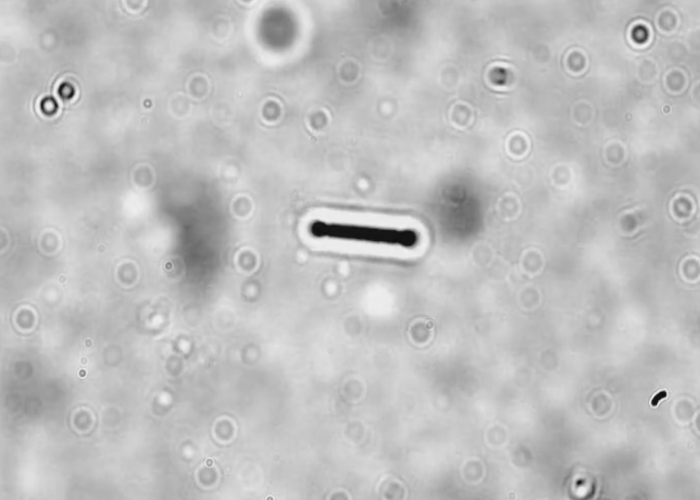
\includegraphics[width=\textwidth]{figures/method/static1.png}
\caption{A typical raw video frame.}\label{fig:origFrame}
\end{subfigure}\hspace{1em}%
\begin{subfigure}[3b]{0.40\textwidth}
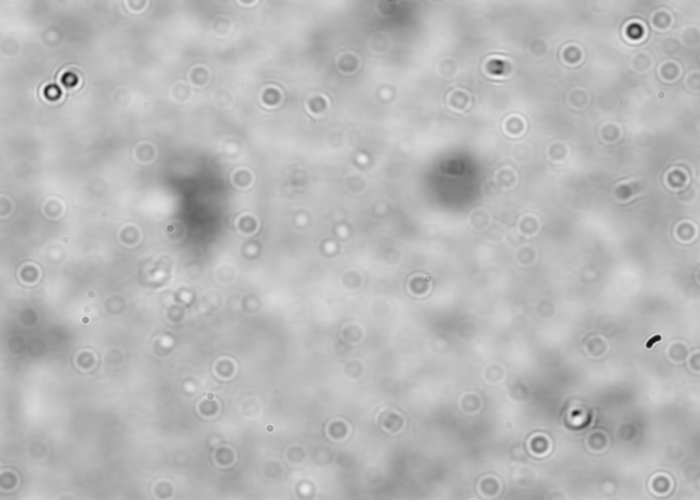
\includegraphics[width=\textwidth]{figures/method/static3.png}
\caption{The average frame $\hat{F}$ from eq \ref{eq:averageFrame}.}\label{fig:averageFrame}
\end{subfigure} \\

\begin{subfigure}[3a]{0.4\textwidth}
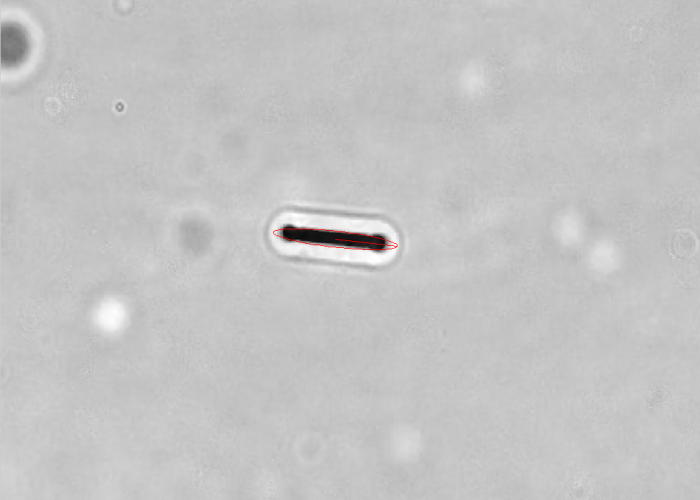
\includegraphics[width=\textwidth]{figures/method/static2.png}
\caption{The same frame after noise reduction}\label{fig:fixedFrame}
\end{subfigure}\hspace{1em}%
\begin{subfigure}[3a]{0.4\textwidth}
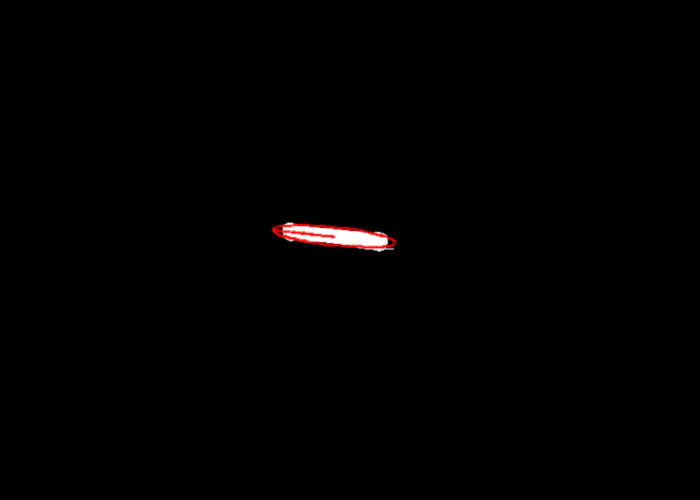
\includegraphics[width=\textwidth]{figures/method/edge.png}
\caption{After edge detection and ellipse fitting}\label{fig:edgeFrame}
\end{subfigure}

\caption{These pictures show a simplified version of the image analysis from raw image to estimated particle position}
\label{fig:detection}
\end{figure}

\section{Estimation of orientation}

The ellipsoid given by the fitting is then our best approximation of the projection of the actual particle. In order to normalize $\mathbf{n}$ we need to know the length of the particle. It was shown by Leal \cite{Leal} that the particle will always spend a majority of its time aligned with the flow, ie aligned with the camera which means that by simply calculating the length $L$ every frame and finding the mode of the distribution we will find a good estimate of L. 

So given an ellipsoid with length $l_e$, width $d_e$ and angle $\phi_p$ we find 

\begin{align} \label{eq:project}
p_x  &= l_e \sin(\phi_p) \\
p_z  &= l_e \cos(\psi_p) 
\end{align}

with x and z projection $p_x$ and $p_z$. To find $\mathbf{n}$ we normalize the projection using
\begin{subequations}\label{eq:normalize}
\begin{align}
n_x 	&= \frac{p_x}{L}, \\
n_z 	&= \frac{p_z}{L}, \\
n_y		&= \sqrt{1 - n_x^2 - n_z^2}.
\end{align}
\end{subequations}


\section{Width compensation}\label{sec:width_compensation}
Up until this point we have assumed that the particle is a \emph{thin} rod so that the projection $\mathbf{p}$ onto the x and z-axes give us an accurate estimate of $\mathbf{n}$. However, when we are projecting a 'thick' particle with length L and width D we get $\mathbf{n}'$. At $\phi = 0$ this is

\begin{equation}
\mathbf{n}' = n_z' = n_z\cos(\theta)  + D\sin(\theta) 
\end{equation}

which is illustrated in figure \ref{fig:lengtherror}. 

In order to compensate for this error we modify our projection equation \ref{eq:project} to

\begin{align}\label{eq:widthCompensation}
p_x  &= (l_e - w_e)\cdot \sin(\phi_p) \\
p_z  &= (l_e - w_e)\cdot \cos(\psi_p) 
\end{align}

This will reduce the particles estimated length by $w_e$
\begin{figure}[H]
\centering
\includegraphics[width=0.6\textwidth]{figures/method/LengthError.pdf}
\caption{Shows the error we get from assuming the particle is thin when it has a width. Shows four different times at $n_x$ = 0. }\label{fig:lengtherror}
\end{figure} 

